\documentclass{article}

%%%%%%%%%%%%%%% LIBRERIAS %%%%%%%%%%%%%%%%%%%%%
\usepackage[thinc]{esdiff}
\usepackage{amsmath}
\usepackage{caption}
\usepackage{physics}
\usepackage{titlesec}
\usepackage{titletoc}
\usepackage{graphicx}
\usepackage[spanish,es-tabla]{babel} % 'es-tabla' cambia Cuadro→Tabla
\usepackage{hyperref}                % cargar después de babel
\usepackage{float}
\usepackage{circuitikz}
\usepackage[left=1.6cm,right=1.6cm,top=1.8cm,bottom=1.8cm]{geometry}
\usepackage{subfiles} 
\usepackage{subcaption}
\usepackage{pgfplots}
\pgfplotsset{compat=1.18}
\usepackage{booktabs} % Para tablas con tematica de paper cientifico
\usepackage{siunitx}  % Para alinear números en las tablas d:

%%%%%%%%%%%%%%%%%%% VARIABLES %%%%%%%%%%%%%%%%%%%%
\newcommand{\Facultad}{Instituto Tecnológico \\de\\ Buenos Aires} %constantes
\newcommand{\TPn}{Trabajo Práctico N° 1}
\newcommand{\TPtema}{Osciloscopios - Analizador de Impedancias}
\renewcommand{\thesection}{\arabic{section}}          % 2
\renewcommand{\thesubsection}{\quad \alph{subsection}}   % a
\renewcommand{\thesubsubsection}{\quad \thesubsection.~\roman{subsubsection}} % a. i
\graphicspath{{imagenes/}} %para que acceda a las fotos en la carpeta directamente


%%%%%%%%%%%%%%%%%% FORMATO TÍTULO Y NUMERACIÓN %%%%%%%%%%%%%%%%%%%
% Numeración de secciones
\renewcommand{\thesection}{\arabic{section}.}          
\renewcommand{\thesubsection}{\thesection\arabic{subsection}}       
\renewcommand{\thesubsubsection}{$\alph{subsubsection})$}

% Numerar hasta subsubsecciones
\setcounter{secnumdepth}{3}

% Formato de títulos
\titleformat{\section}{\Huge\bfseries}{\thesection}{1em}{}
\titleformat{\subsection}{\LARGE\bfseries}{\thesubsection}{0.5em}{}
\titleformat{\subsubsection}{\large\bfseries}{\thesubsubsection}{0.5em}{}



%%%%%%%%%%%%%%%%%%% ARCHIVO %%%%%%%%%%%%%%%%%%%%%%%%
\begin{document}

%%%CARATULA%%%
\begin{titlepage} %creo portada

        \begin{flushleft}
            \centering
            
\includegraphics[width=0.3\textwidth]{Logo_ITBA.png}
        \end{flushleft}

        \centering
            
        {\scshape\LARGE \Facultad \par} %\par sirve para indicar un final de parrafo
        \vspace{1cm}                    %esto hace un espacio entre lineas de 1cm


        {\huge\bfseries \TPn \par}
        \vspace{1.5cm}
        {\Large Laboratorio de Electrónica\\ 25.13 \par}
        \vspace{0.5cm}
        {\Large \TPtema \par}
        \vfill                      %sirve para rellenar el espacio y quede simétrico.
        {\Large \bfseries Grupo N° 2 \par}
        \vspace{1cm}
        {\large Juan Bautista Correa Uranga \hfill Legajo: 65016 \par} 
        {\large Juan Ignacio Caorsi \hfill Legajo: 65532  \par}
        {\large Rita Moschini \hfill Legajo: 67026 \par} 
        {\large Lucas Solar Grillo \hfill Legajo: 63322\par}
        \vfill
        {\large \today\par}
        \vfill

\end{titlepage}

{\centering \LARGE \bfseries Resumen \par} 
\par 

\newpage

\tableofcontents 
\newpage

%%%%%%%%%%%%%%%%%%% CUERPO DEL INFORME %%%%%%%%%%%%%%%%%%%%%%%%

\section{Objetivos}
El objetivo de este trabajo práctico es utilizar circuitos RC de primer orden, en configuraciones pasabajos y pasaaltos, como base para analizar el uso del instrumental de laboratorio en condiciones reales. Dado que su comportamiento teórico es conocido, se los emplea como referencia para comparar con las mediciones experimentales e identificar las diferencias que aparecen en la práctica. En particular, se busca trabajar con herramientas como el generador de señales, el osciloscopio digital y la función de Network Analyzer, poniendo foco en cómo las condiciones de medición afectan los resultados, considerando efectos como la resistencia de salida del generador, la impedancia de entrada del osciloscopio y las capacitancias parásitas de las puntas. Finalmente, se pretende interpretar las diferencias entre los resultados teóricos y experimentales, teniendo en cuenta tanto las tolerancias de los componentes como las limitaciones del instrumental.

\section{Instrumentos y equipo}
    \begin{itemize}
        \item Protoboard de 830 puntos
        \item Capacitor de 3,4 nF
        \item Resistencia de 4,6 k$\Omega$
        \item Osciloscopio digital Keysight DSOX1202G
        \item Generador de señales Picotest G510
        \item Generador de señales Keysight EDU33212A
        \item Medidor RLC UNI-T UT812
    \end{itemize}

    \newpage
\section{Pasa bajos}
    \subsection{Parte teórica}
        % a) Transferencia y frecuencia de corte
        % b) Frecuencia nominal y error
        % c) Ángulo de fase y diagrama vectorial
        % d) Diagrama de Bode teórico con tolerancias
        % e) Ganancia y fase para fo/10, fo y 10fo
        % f) Simulación con onda cuadrada
    a) Para este circuito, se llega a la siguiente ecuación: 
    \begin{equation}
H(s)=\frac{1}{\frac{s}{\frac{1}{R \cdot C}}+1}
\label{eq:pasabajos}
\end{equation}

    (Observar deduccion \ref{subsec:decuccion filtros}).\\
    De esta ecuación se obtiene la frecuencia de corte $ f_0 = \frac{1}{2 \cdot \pi \cdot R \cdot C} $. Finalmente, remplazando los valores de los componentes se obtiene la frecuencia de corte teorica: $f_0= 10261 Hz$. 
    

	b) Para este circuito se utilizaron una $R = 4,7 k\Omega \pm 5 \%$ y un $C = 3,3 nF \pm 10\%$. \par
	De esta manera la frecuencia de resonancia con su error sería $f_0 = 10261 Hz \pm 1147 Hz$. (Observar deducción \ref{subsec: Deducción del error de la frecuencia})

	
	c) Puesto a que el circuito es una malla, todos sus componentes poseen la misma $I$. Luego la la diferencia de fase está dada por $\angle V_c - \angle I = -90$. (Observar deducción \ref{subsec:desfase}). \par 
	
	Se calcularon los valores de la corriente y tensión teóricos usando los valores nominales y teniendo en cuenta los 50 ohms de la entrada del generador. $I=  0,75mA \angle 44,69$ y $V_c = 3,52 V \angle -45,30$. Observemos que se cumple el desfase de -90. (Observar figura \ref{fig:fasorial}).
	
	
	%%%%%nuevo%%%%%
	\begin{figure}[H]
\centering

\begin{minipage}{0.48\textwidth}
\centering
{
\shorthandoff{<>}
\begin{tikzpicture}[scale=0.5]

    % Ejes
    \draw[->] (-0.5,0) -- (4.5,0) node[right] {$\Re$};
    \draw[->] (0,-3.5) -- (0,3.5) node[above] {$\Im$};

    % Corriente
    \draw[->, thick] (0,0) -- (44.69:2.0)
        node[above right] {$\vec{I}=0.75\,\mathrm{mA}\angle 44.69^\circ$};

    % Tensión capacitor
    \draw[->, thick] (0,0) -- (-45.3:3.0)
        node[below right] {$\vec{V}_C=3.52\,\mathrm{V}\angle -45.3^\circ$};

\end{tikzpicture}
}
\captionof{figure}{Diagrama fasorial representativo (no a escala entre magnitudes de distinta unidad).}
\label{fig:fasorial}
\end{minipage}
\hfill
\begin{minipage}{0.48\textwidth}
\centering
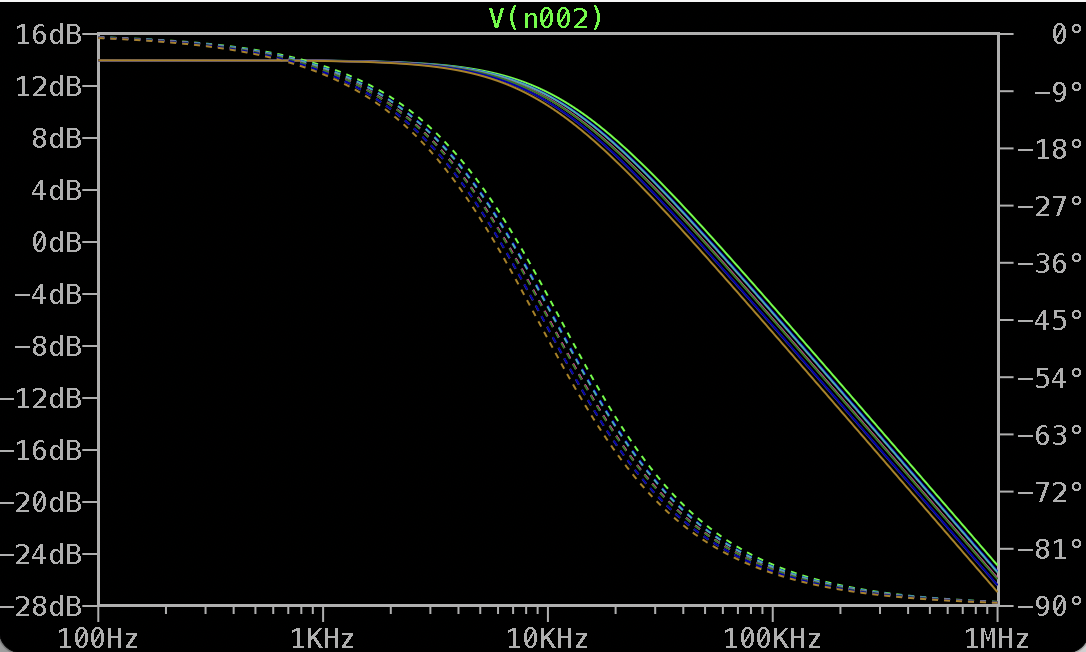
\includegraphics[width=0.85\textwidth]{1.1d}
\captionof{figure}{Diagrama de Bode posibles tomando valor máximo, nominal y mínimo de los componentes.}
\label{fig:bode1.1d}
\end{minipage}

\end{figure}
%%%%%%nuevo%%%%%

	
	
	En segundo lugar, se verificará la expresión $ \vec{V_R} + \vec{V_C} = \vec{V}$. Para realizar esto, se realizará de manera algebraica para todos los valores. $ V = I \cdot Z = I (R + \frac{1}{j \cdot \omega}) = I\cdot R + \frac{I}{j \cdot \omega} = V_R + V_C$.

d) Para esta parte, se realizo el diagrama del bode del circuito, combinando todos los casos posibles, considerando los valores mínimos, nominales y máximos de los componentes. 

e) De la ecuación \ref{eq:pasabajos}, se despejaron los siguientes valores:

Para $\frac{f_0}{10}$, se observó una atenuación de 1,1 veces o lo mismo que $-0,04 dB \approx 0 db$. Luego $\angle H(\frac{f_0}{10}) = -5,71^\circ$.\\

 Para $f_0$, se observó una atenuación de 2 veces la señal de entrada, o lo mismo que $-3 dB$. Luego se despejo $\angle H(f_0) = -45^\circ$.\\
 
 Para $10 \cdot f_0$, se observó una atenuación de 10 veces la señal de entrada, o lo mismo que $-20 db$. Luego se despejó $\angle H(10 \cdot f_0) = -84,29 ^\circ$.\\
 

f) Para esta parte, se simularon los tres casos (Observar imagenes \ref{fig:20f0}, \ref{fig:f0} y \ref{fig:f0sobre20}).

\begin{figure}[h!]
    \centering
    
    \begin{minipage}{0.32\textwidth}
        \centering
        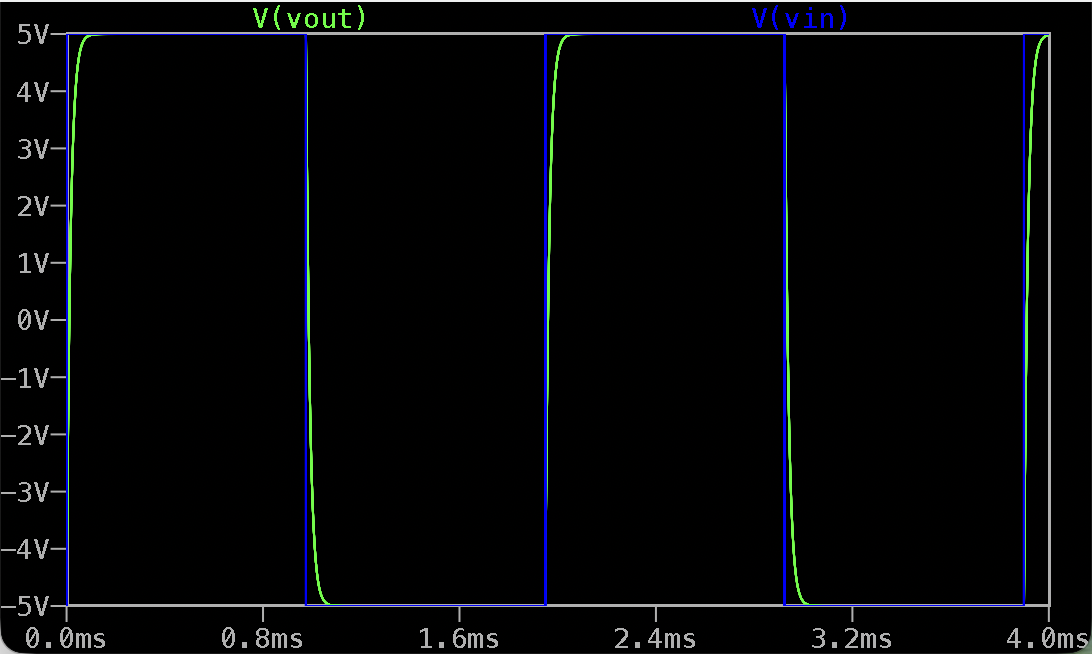
\includegraphics[width=\textwidth]{1.1f(f0sobre20)}
        \caption{Gráfico con $f=\frac{f_0}{20}$.}
        \label{fig:f0sobre20}
    \end{minipage}
    \hfill
    \begin{minipage}{0.32\textwidth}
        \centering
        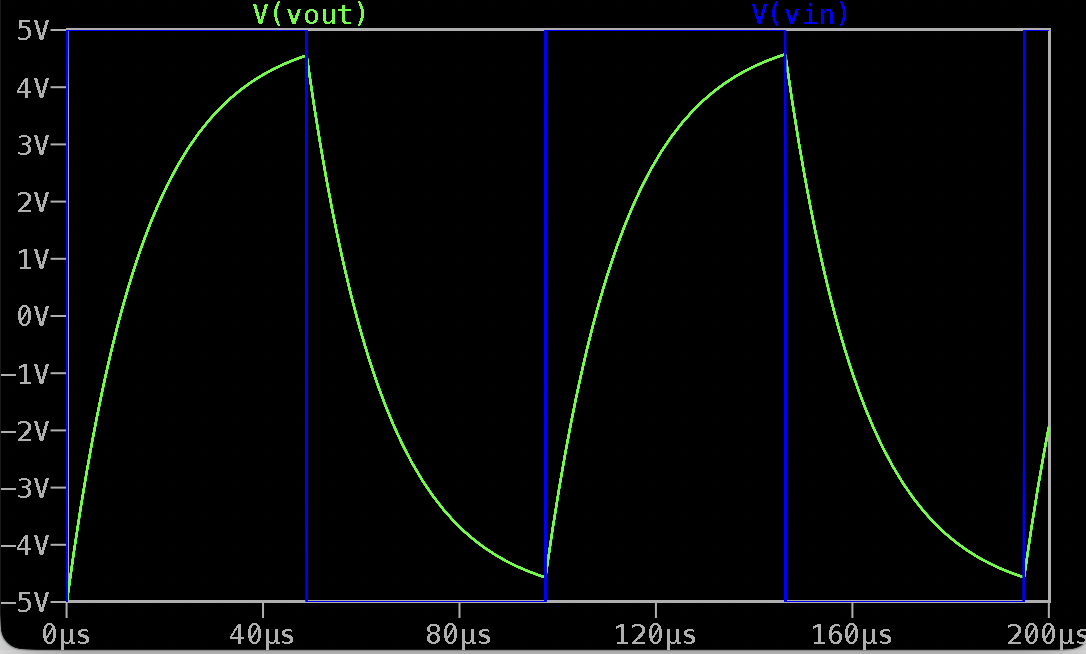
\includegraphics[width=\textwidth]{1.1f(f0)}
        \caption{Gráfico con $f=f_0$.}
        \label{fig:f0}
    \end{minipage}
    \hfill
    \begin{minipage}{0.32\textwidth}
        \centering
        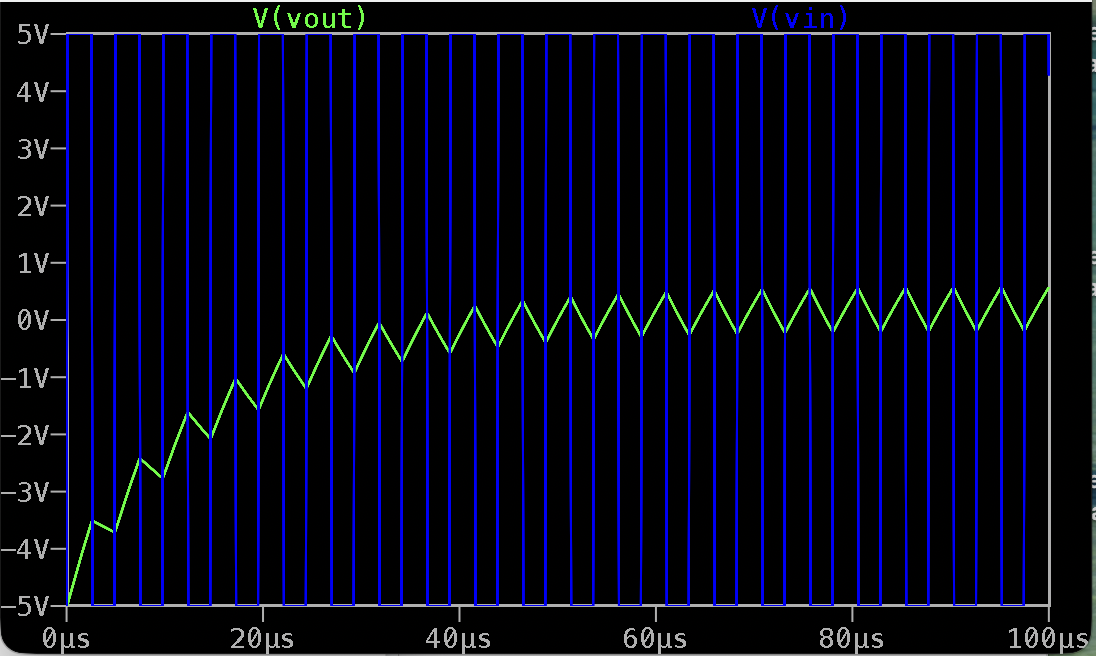
\includegraphics[width=\textwidth]{1.1f(f0.20)}
        \caption{Gráfico con $f=20\,f_0$.}
        \label{fig:20f0}
    \end{minipage}
    
\end{figure}

Al observar los gráficos se puede observar que $v_{out}$ se termina comportando como una respuesta transitoria RC. Al inicio de la señal el circuito se carga de forma exponencial, y luego se descarga en forma exponencial. \par

En el caso de $f=\frac{f_0}{20}$, el circuito tiene mucho tiempo prendido o apagado en comparación al tiempo de carga del capacitor, por lo que se puede apreciar perfectamente los pasos de carga y descarga de un RC. Luego en el caso de $f=f_0$, el circuito se sigue comportando como un sistema RC. Ahora cuando aumentamos la frecuencia a $f=20\cdot f_0$, el tiempo de carga y descarga es tan chicho en comparación a la señal de entrada que no se logra observar una forma exponencial de un RC. En este caso decimos que el sistema aproxima a un integrador, puesto a que se conforma casi de forma linean en la carga y en la descarga.

De manera analitica:

\begin{align*}
    H(s) &= \frac{V_{out}}{V_{in}}      \qquad    \Rightarrow V_{out}=V_{in} \cdot \frac{1}{1+sCR}\\
    Pero\ como &\ \frac{f}{f_0}>> 1\ ,desprecio +1       \qquad     \Rightarrow V_{out}=V_{in} \cdot \frac{1}{sCR}\\
    Luego\ antitransfo&rmando\ y\ recordando\ la\ propiedad,         \qquad      y(t)=h(t) * x(t)       \qquad      \Rightarrow y(t)=\frac{1}{RC} \cdot \int_{}^{}x(t)\\
\end{align*}



    \subsection{Parte práctica}
                % a) Frecuencia de corte real y cálculo de C
                        \subsubsection*{a) Frecuencia de corte real y cálculo de C}
        
                    Para determinar la frecuencia de corte real del circuito, se alimentó el sistema
                     con una señal senoidal con una amplitud nominal de $5\text{ V}$. Durante
                      la medición en la frecuencia de corte, se registró un voltaje de entrada
                       de $|V_{in}| = 5,1\text{ V}$ y un voltaje de salida sobre el capacitor 
                       de $|V_c| = 3,535\text{ V}$. Estos valores se corresponden con el punto 
                       de operación donde se espera obtener una atenuación de $-3\text{ dB}$.
                    Se elige la señal senoidal de la amplitud mencionada pues se consideró que 
                    sería suficientemente intensa para poder realizar las mediciones sin ruido
                     que afecte la medición de manera significativa.
        
        
                    Es necesario considerar la resistencia total del circuito $R$,
                     la cual resulta de la suma de la resistencia interna de la fuente de señal
                      ($50\ \Omega$) y el valor del resistor del circuito ($4,6\text{ k}\Omega$).
                    Experimentalmente, se determinó que la frecuencia de corte es $f_c = 10,05\text{ kHz}$. Despejando 
                    la capacitancia $C$ de la ecuación $ f_0 = \frac{1}{2 \cdot \pi \cdot R \cdot C} $ y reemplazando con los valores de $R$ y $f_c$ obtenidos, se obtiene $C \approx 3,41\text{ nF}$.

                % b) Ángulo de fase medido vs teórico
                \subsubsection*{b) Ángulo de fase medido vs teórico}
        
                    Se midió experimentalmente la diferencia de fase entre la corriente $i$
                     y la tensión sobre el capacitor $v_c$.
        
                    El valor medido en la práctica fue de $-88,5^\circ$. Esta pequeña diferencia
                     de $1,5^\circ$ respecto al valor ideal se puede atribuir a que la medición de desfase del osciloscopio
                         puede presentar incertezas del orden de $\pm 1^\circ$; 
        

                % c) Tabla de valores en frecuencia (10Hz a 1MHz)
                \subsubsection*{c) Tabla de valores en frecuencia (10 Hz a 1 MHz)}
        
                    Se excitó el circuito con una onda sinusoidal variando la frecuencia para caracterizar la función de transferencia del filtro. 
                    En el anexo se presenta la tabla con los valores experimentales medidos y calculados.
        
                    Es importante destacar que las mediciones se detuvieron en la década 
                    correspondiente a $100\text{ kHz}$. Considerando que luego de una década de la frecuencia de corte el ángulo de la función de transferencia ($H$)
                     se mantiene prácticamente asintótico, al igual que la tasa de decaimiento de su módulo ($|H|$) que adopta una pendiente constante, se evaluó que los puntos elegidos son los que más valor aportan para trazar la curva. Esto permite obtener una correcta apreciación del comportamiento del filtro mucho antes de alcanzar la frecuencia máxima sugerida de $1\text{ MHz}$. 
                % d) Diagrama de Bode superpuesto
                \subsubsection*{d) Diagrama de Bode superpuesto}
                En base a los datos recolectados en la tabla \ref{tab:pasa_bajos_freq}, se graficó los puntos correspondientes sobre el diagrama de Bode teórico obtenido en el punto 1.1.d).

                Se ven ciertas desviaciones al final, solo se pueden explicar en su mayoría por error de medición. Luego, la desviación que se ve en el resto de los puntos respecto a una u otra curva teórica se debe a la tolerancia de los componentes.
                % e) Diagrama de Bode con Network Analyzer
                \subsubsection*{e) Diagrama de Bode con Network Analyzer}
        
                Utilizando la función de Análisis de Respuesta en Frecuencia (FRA) del osciloscopio, se obtuvo el diagrama de Bode empírico del circuito pasa-bajos (ver en anexos).

                Al analizar la Figura \ref{fig:bode_tikz_final}, se confirman de manera visual e instrumental los resultados esperados: la atenuación de $-3\text{ dB}$ y el desfase cruzando por $-45^\circ$ en las cercanías de la frecuencia de corte, seguido por la caída asintótica de la ganancia a $-20\text{ dB/década}$ y el límite de fase hacia los $-90^\circ$.
        
        
                
                % f) Gráficos de onda cuadrada
        
                \subsubsection*{f) Gráficos de onda cuadrada y conclusiones temporales}
        
                    Para evaluar la respuesta transitoria del sistema, 
                    se reemplazó la señal de entrada por una onda cuadrada de $10\text{ V}_{pp}$,
                     variando su frecuencia dentro del rango de estudio. Se capturaron las formas
                      de onda a la salida (sobre el capacitor) para tres frecuencias representativas:
                       $100\text{ Hz}$, $1\text{ kHz}$ y $10\text{ kHz}$ (ver en anexos).
        

                    Al analizar los oscilogramas obtenidos (Figura \ref{fig:ondas_cuadradas}), se extraen las siguientes conclusiones:
        %oscilograma: representación gráfica de una señal eléctrica en función del tiempo, obtenida mediante un osciloscopio
                    \begin{itemize}
                        \item \textbf{A bajas frecuencias (100 Hz):} El
                         tiempo prendido de la señal cuadrada es muchísimo
                          mayor que la constante de tiempo del circuito ($\tau = RC$).
                           El capacitor tiene tiempo de sobra para cargarse y descargarse por completo.
                            Por lo tanto, la señal de salida copia casi fielmente a la entrada.
                        \item \textbf{A frecuencias medias (1 kHz):} 
                        El tiempo prendido de la señal ahora comienza a 
                        acercarse a la constante de tiempo. Se hace claramente 
                        visible el régimen transitorio (la curva exponencial de carga y descarga 
                        del capacitor). No obstante, la señal aún logra alcanzar el estado estacionario.
                        \item \textbf{En la frecuencia de corte (10 kHz):} 
                        El período de la señal es tan corto que el capacitor no tiene tiempo
                         suficiente para alcanzar su nivel de carga máximo ni para descargarse
                          por completo. La señal de salida pierde por completo su forma cuadrada 
                          y sufre una atenuación en amplitud. Si siguiera aumentando la frecuencia es esperable que la salida se acerque cada vez más a una triangular.
                    \end{itemize}
                    % g) Cálculo de vr y gráfico
                \subsubsection*{g) Cálculo y gráfico de la tensión en la resistencia ($|v_r|$)} \label{vr}
        
        A partir de los módulos medidos, se calculó la tensión en la resistencia:
        $$|v_r| = \sqrt{|v|^2 - |v_c|^2}$$
        
        Los resultados obtenidos para cada frecuencia se detallan en la tabla \ref{tab:vr_calculada}(ver en anexos). 
    
        
        Luego, se presenta el gráfico de la tensión $|v_r|$ en función de la frecuencia, utilizando una escala logarítmica para el eje de frecuencias.
        
\begin{figure}[H]
    \centering
    \begin{tikzpicture}
        \begin{semilogxaxis}[
            width=7cm, height=3.5cm, % <-- tamaño reducido
            title={Tensión en la resistencia ($|v_r|$) vs. Frecuencia},
            xlabel={Frecuencia [Hz]},
            ylabel={Tensión $|v_r|$ [V]},
            xmin=100, xmax=100000,
            ymin=0, ymax=5.5,
            ytick={0, 1, 2, 3, 4, 5},
            grid=both,
            grid style={line width=.1pt, draw=gray!30},
            major grid style={line width=.2pt,draw=gray!50},
            axis lines=left,
            every axis plot/.append style={thick}
        ]

            \addplot[
                color=blue,
                mark=*,
                mark size=2.4pt,
                only marks
            ] coordinates {
                (500, 0.71) (1000, 0.71) (2000, 1.00) (5000, 2.29) 
                (7000, 2.88) (10000, 3.59) (15000, 4.20) (20000, 4.52) 
                (25000, 4.68) (30000, 4.74) (35000, 4.81) (40000, 4.81) 
                (45000, 4.84) (50000, 4.90) (55000, 4.91) (60000, 4.92) 
                (65000, 4.93) (70000, 4.94) (75000, 5.00) (80000, 4.95) (100000, 5.02)
            };

        \end{semilogxaxis}
    \end{tikzpicture}
    \caption{Puntos experimentales de la tensión sobre la resistencia en función de la frecuencia.}
    \label{fig:vr_grafico_puntos}
\end{figure}
        A partir del gráfico y de los datos calculados, se ve que en la frecuencia de corte $f_c \approx 10\text{ 10 kHz}$, se observa que las tensiones $v_r$ y $v_c$ son prácticamente iguales ($3,59\text{ V}$ y $3,55\text{ V}$, respectivamente). Esto demuestra físicamente que, en este punto exacto, el módulo de la reactancia capacitiva ($X_C$) se iguala al valor de la resistencia ($R$).
        Además, se ve que al poner el foco en la caída de tensión de la resistencia, se evidencia que la mayor parte de la tensión de la fuente cae sobre ella únicamente cuando las frecuencias son altas. Por lo tanto, si se toma la salida sobre la resistencia en lugar del capacitor, el circuito se comporta como un filtro pasa-altos.

        % h) Medición sin C (x1 y x10)
        \subsubsection*{h) Caracterización de la capacitancia de la punta ($C_p$)}

Se procedió a repetir el ensayo de respuesta en frecuencia retirando el capacitor físico del circuito RC, de modo que la carga reactiva quedó constituida únicamente por el conjunto punta-osciloscopio.
Repitiendo los cálculos y mediciones realizados en el punto 4.2.a), se obtiene $C_{punta x1}$ y $C_{punta x10}$.
Ver el desarrollo detallado en el anexo.
Se obtuvo que $C_{punta x1} \approx 114\text{ pF}$ y $C_{punta x10} \approx 17\text{ pF}$, lo cual se encuentra dentro de los valores típicos esperados para cada modo de la punta. Esto confirma que el conjunto punta-osciloscopio introduce una capacitancia parásita significativa, especialmente en modo X1, que puede afectar las mediciones a frecuencias más altas.

 % i) Conclusiones de esta sección
\subsubsection*{i) Conclusiones}
Se concluyó que es necesario considerar evaluar el efecto que tiene el conjunto osciloscopio-punta
pues según el valor de los componentes dentro de cualquier circuito a estudiar, estos pueden ocasionar errores apreciables.

               
%%%%%%%%%
%%%%%%%%%

\section{Pasa altos}
    \subsection{Parte teórica}
        \subsubsection{Transferencia y frecuencia de corte}
            Para este circuito, se llega a la siguiente ecuación: 
    \begin{equation}
H(s)=\frac{sRC}{\frac{s}{\frac{1}{R \cdot C}}+1}
\label{eq:pasaaltos}
\end{equation}

    (Observar deduccion \ref{subsec:decuccion filtros}).\\
    De esta ecuación se obtiene la frecuencia de corte $ f_0 = \frac{1}{2 \cdot \pi \cdot R \cdot C} $. Finalmente, remplazando los valores de los componentes se obtiene la frecuencia de corte teorica: $f_0= 10261 Hz$. Observesé que la frecuencia de corte coincide con la del pasa bajos.
        \subsubsection{Frecuencia nominal y error}
            El analisis en de la frecuencia de corte y error es homologo al de la sección 1.1.b.\par
            
            Por tal motivo resulta quedando $f_0 = 10261 Hz \pm 1147 Hz$.
    \subsubsection{Diagrama de Bode con tolerancias}         
            %%%%%

\begin{figure}[H]
\centering

\begin{minipage}{0.48\textwidth}
\centering
\begin{tikzpicture}
\begin{semilogxaxis}[
    xlabel={Frecuencia [Hz]},
    ylabel={Ganancia [dB]},
    grid=both,
    width=\textwidth,
    height=6cm,
    xmin=100, xmax=2e5,
    ymin=-40, ymax=5,
    legend pos=south east
]

% Nominal
\addplot[
    domain=100:2e5,
    samples=200,
    thick,
    blue
]
{20*log10( (2*pi*x*4.7e3*3.3e-9) / sqrt(1+(2*pi*x*4.7e3*3.3e-9)^2) )};
\addlegendentry{Nominal}

% Mínimo
\addplot[
    domain=100:2e5,
    samples=200,
    thick,
    red,
    dashed
]
{20*log10( (2*pi*x*(4.7e3*1.05)*(3.3e-9*1.10)) / sqrt(1+(2*pi*x*(4.7e3*1.05)*(3.3e-9*1.10))^2) )};
\addlegendentry{Mínimo}

% Máximo
\addplot[
    domain=100:2e5,
    samples=200,
    thick,
    green!60!black,
    dashed
]
{20*log10( (2*pi*x*(4.7e3*0.95)*(3.3e-9*0.90)) / sqrt(1+(2*pi*x*(4.7e3*0.95)*(3.3e-9*0.90))^2) )};
\addlegendentry{Máximo}

% Líneas verticales
\addplot[dotted, thick] coordinates {(8884,-40) (8884,5)};
\addplot[dotted, thick] coordinates {(10261,-40) (10261,5)};
\addplot[dotted, thick] coordinates {(12000,-40) (12000,5)};

\end{semilogxaxis}
\end{tikzpicture}
\end{minipage}
\hfill
\begin{minipage}{0.48\textwidth}
\centering
\begin{tikzpicture}
\begin{semilogxaxis}[
    xlabel={Frecuencia [Hz]},
    ylabel={Fase [°]},
    grid=both,
    width=\textwidth,
    height=6cm,
    xmin=100, xmax=2e5,
    ymin=0, ymax=100,
    legend pos=south west
]

% Nominal
\addplot[
    domain=100:2e5,
    samples=200,
    thick,
    blue
]
{atan(1/(2*pi*x*4.7e3*3.3e-9))};
\addlegendentry{Nominal}

% Mínimo
\addplot[
    domain=100:2e5,
    samples=200,
    thick,
    red,
    dashed
]
{atan(1/(2*pi*x*(4.7e3*1.05)*(3.3e-9*1.10)))};
\addlegendentry{Mínimo}

% Máximo
\addplot[
    domain=100:2e5,
    samples=200,
    thick,
    green!60!black,
    dashed
]
{atan(1/(2*pi*x*(4.7e3*0.95)*(3.3e-9*0.90)))};
\addlegendentry{Máximo}

% Líneas verticales
\addplot[dotted, thick] coordinates {(8884,0) (8884,100)};
\addplot[dotted, thick] coordinates {(10261,0) (10261,100)};
\addplot[dotted, thick] coordinates {(12000,0) (12000,100)};

\end{semilogxaxis}
\end{tikzpicture}
\end{minipage}

\caption{Diagramas de Bode del filtro pasaaltos considerando valores nominales, mínimos y máximos de los componentes.}
\end{figure}
            
            %%%%

    \subsubsection{Ganancia y fase en distintas frecuencias con una sinosoidal}
            De la ecuación \ref{eq:pasaaltos} se despejaron los siguientes valores evaluando en las frecuencias solicitadas:\par


            Para $f=\frac{f_0}{10}$: $|H| \approx 0.0995 \quad \Rightarrow \quad 20\log_{10}|H| \approx -20\,\text{dB}$ y fase $\angle H \approx 84.3^\circ$
                

            Para $f=f_0$:  $|H|=\frac{1}{\sqrt{2}} \approx 0.707 \quad \Rightarrow \quad -3\,\text{dB}$ y fase $\angle H = 45^\circ$


            Para $f=10f_0$: $  |H| \approx 0.995 \quad \Rightarrow \quad 0\,\text{dB}$ y fase $\angle H \approx 5.7^\circ$

    \subsubsection{Simulacion de una entrada de onda triangular}
    
    %%%%nuevo%%%%%
\begin{figure}[H]
    \centering

    % ---------- fila superior ----------
    \begin{minipage}[t]{0.45\textwidth}
    \centering
    \begin{tikzpicture}
    \begin{axis}[
        width=0.9\textwidth,
        height=3.8cm,
        scale only axis,
        grid=both,
        xlabel={Tiempo [s]},
        ylabel={Tensión [V]},
        legend pos=north east,
        no marks
    ]

    \addplot table [x=time, y=V(n001), col sep=tab] {10fo.txt};
    \addlegendentry{Entrada}

    \addplot table [x=time, y=V(a), col sep=tab] {10fo.txt};
    \addlegendentry{Salida}

    \end{axis}
    \end{tikzpicture}
    \captionof{figure}{Filtro pasa-altos para $f = 10 f_0$.}
    \label{fig:10f0}
    \end{minipage}
    \hfill
    %
    \begin{minipage}[t]{0.45\textwidth}
    \centering
    \begin{tikzpicture}
    \begin{axis}[
        width=0.9\textwidth,
        height=3.8cm,
        scale only axis,
        grid=both,
        xlabel={Tiempo [s]},
        ylabel={Tensión [V]},
        legend pos=north east,
        no marks
    ]

    \addplot table [x=time, y=V(n001), col sep=tab] {fo.txt};
    \addlegendentry{Entrada}

    \addplot table [x=time, y=V(a), col sep=tab] {fo.txt};
    \addlegendentry{Salida}

    \end{axis}
    \end{tikzpicture}
    \captionof{figure}{Filtro pasa-altos para $f = f_0$.}
    \label{fig:f0}
    \end{minipage}

    \vspace{0.35cm}

    % ---------- fila inferior ----------
    \begin{minipage}{0.5\textwidth}
    \centering
    \begin{tikzpicture}
    \begin{axis}[
        width=0.9\textwidth,
        height=3.8cm,
        scale only axis,
        grid=both,
        xlabel={Tiempo [s]},
        ylabel={Tensión [V]},
        legend pos=north east,
        no marks
    ]

    \addplot table [x=time, y=V(n001), col sep=tab] {fo_10.txt};
    \addlegendentry{Entrada}

    \addplot table [x=time, y=V(a), col sep=tab] {fo_10.txt};
    \addlegendentry{Salida}

    \end{axis}
    \end{tikzpicture}
    \captionof{figure}{Filtro pasa-altos para $f = \frac{f_0}{10}$.}
    \label{fig:f0_10}
    \end{minipage}

\end{figure}

    %%%%nuevo%%%%%

    \subsubsection{Análisis analítico para entrada triangular}
	\label{subsec:deduccion analitica derivador}

        El circuito bajo análisis es un sistema lineal e invariante en el tiempo (LTI), por lo que su salida puede expresarse como la convolución entre la señal de entrada y la respuesta impulsiva del sistema:

        \begin{equation*}
            v_{out}(t) = h(t) * v_{in}(t) \quad \implies V_{out}(s) = H(s)\,V_{in}(s)
        \end{equation*}

        donde $h(t)$ es la respuesta al impulso del sistema.
        
        %%% nuevo%%%
        Para una señal triangular, cada tramo puede aproximarse como:

\[
v_{in}(t) = k t \quad \Rightarrow \quad V_{in}(s) = \frac{k}{s^2}
\]

En el régimen en el cual el circuito se comporta como derivador (bajas frecuencias):
\[
H(s) \approx sRC \qquad \Rightarrow \qquad V_{out}(s) \approx (sRC)\frac{k}{s^2} = \frac{kRC}{s}
\]

Aplicando transformada inversa: $ v_{out}(t) = kRC $

Homologamente para el tramo decreciente: $ v_{out}(t) = -kRC$

Por lo tanto, la salida es una señal cuadrada, verificándose que: 
$v_{out}(t) \approx RC \frac{d}{dt} v_{in}(t) $

lo que demuestra el comportamiento derivador del filtro pasa-altos en este régimen.
        %%%nuevo%%%
    %
    %
    %
    %
    %
    %
    %
    %
    %
    %
    %
    %

%
        
    \subsection{Parte práctica}
        \subsubsection*{a) Diagrama de Bode}
            Una fuente de problemas común al momento de estudiar circuitos es la forma en que los instrumentos de medición afectan a las propias mediciones. En el caso del filtro pasaaltos, se pueden modelar las impedancias del osciloscopio y de las puntas en conjunto agregando en paralelo a la salida un capacitor de $ 100 pF $  y una resistencia de $1 M\Omega$, como se puede observar en la figura \ref{fig:pasaaltosSimulado}.


%%%%imagen no usada, dejo por las dudas%%%%%
 %           \begin{figure}[H]
    %            \centering
    %            \begin{tikzpicture}
   %                 % Paths, nodes and wires:
  %                  \draw (6, 3) to[capacitor] (8, 3);
  %                  \draw (9, 3) to[american resistor] (9, -0);
  %                  \draw (11, 3) to[capacitor] (11, -0);
  %                  \draw (12.75, 3) to[american resistor] (12.75, -0);
   %                 \draw (5, 3) to[sinusoidal voltage source] (5, 0);
    %                \draw (12.75, -0) |- (5, -0);
    %                \node[shape=rectangle, minimum width=1.465cm, minimum height=0.715cm] at (7.25, 3.625){} node[anchor=north west, align=left, text width=1.077cm, inner sep=6pt] at (6.5, 4){3,3n};
 %                   \node[shape=rectangle, minimum width=1.465cm, minimum height=0.715cm] at (8.5, 1.375){} node[anchor=north west, align=left, text width=1.077cm, inner sep=6pt] at (7.75, 1.75){4,7k};
  %                  \node[shape=rectangle, minimum width=1.465cm, minimum height=0.715cm] at (10.75, 1.875){} node[anchor=north west, align=left, text width=1.077cm, inner sep=6pt] at (10, 2.25){100p};
    %                \draw (5, 3) -- (6, 3);
       %             \draw (8, 3) -- (12.75, 3);
       %             \node[shape=rectangle, minimum width=1.465cm, minimum height=0.715cm] at (13.75, 1.5){} node[anchor=north west, align=left, text width=1.077cm, inner sep=6pt] at (13, 1.875){1M};
          %          \node[circ] at (12.75, 3){};
             %       \node[shape=rectangle, minimum width=1.465cm, minimum height=0.715cm] at (13.5, 3){} node[anchor=north west, align=left, text width=1.077cm, inner sep=6pt] at (12.75, 3.375){Vout};
                %\end{tikzpicture}
  %              \caption{Modelo de  filtro pasaaltos considerando las impedancias del osciloscopio y de las puntas.}
 %               \label{fig:pasaaltosNoIdeal}
    %        \end{figure}

            Sin embargo, en este circuito esas no-idealidades afectan poco al comportamiento en frecuencia del mismo. Para las resistencias, la resistencia de $1 M\Omega$ queda en paralelo a la de $4k7\Omega$, y se tiene que la resistencia equivalente vale $\approx 4,7k\Omega$ puesto que $4,7k \ll 1M$, por lo que la resistencia de $ 1 M\Omega$ resulta despreciable.

            \begin{figure}[H]
                \centering
                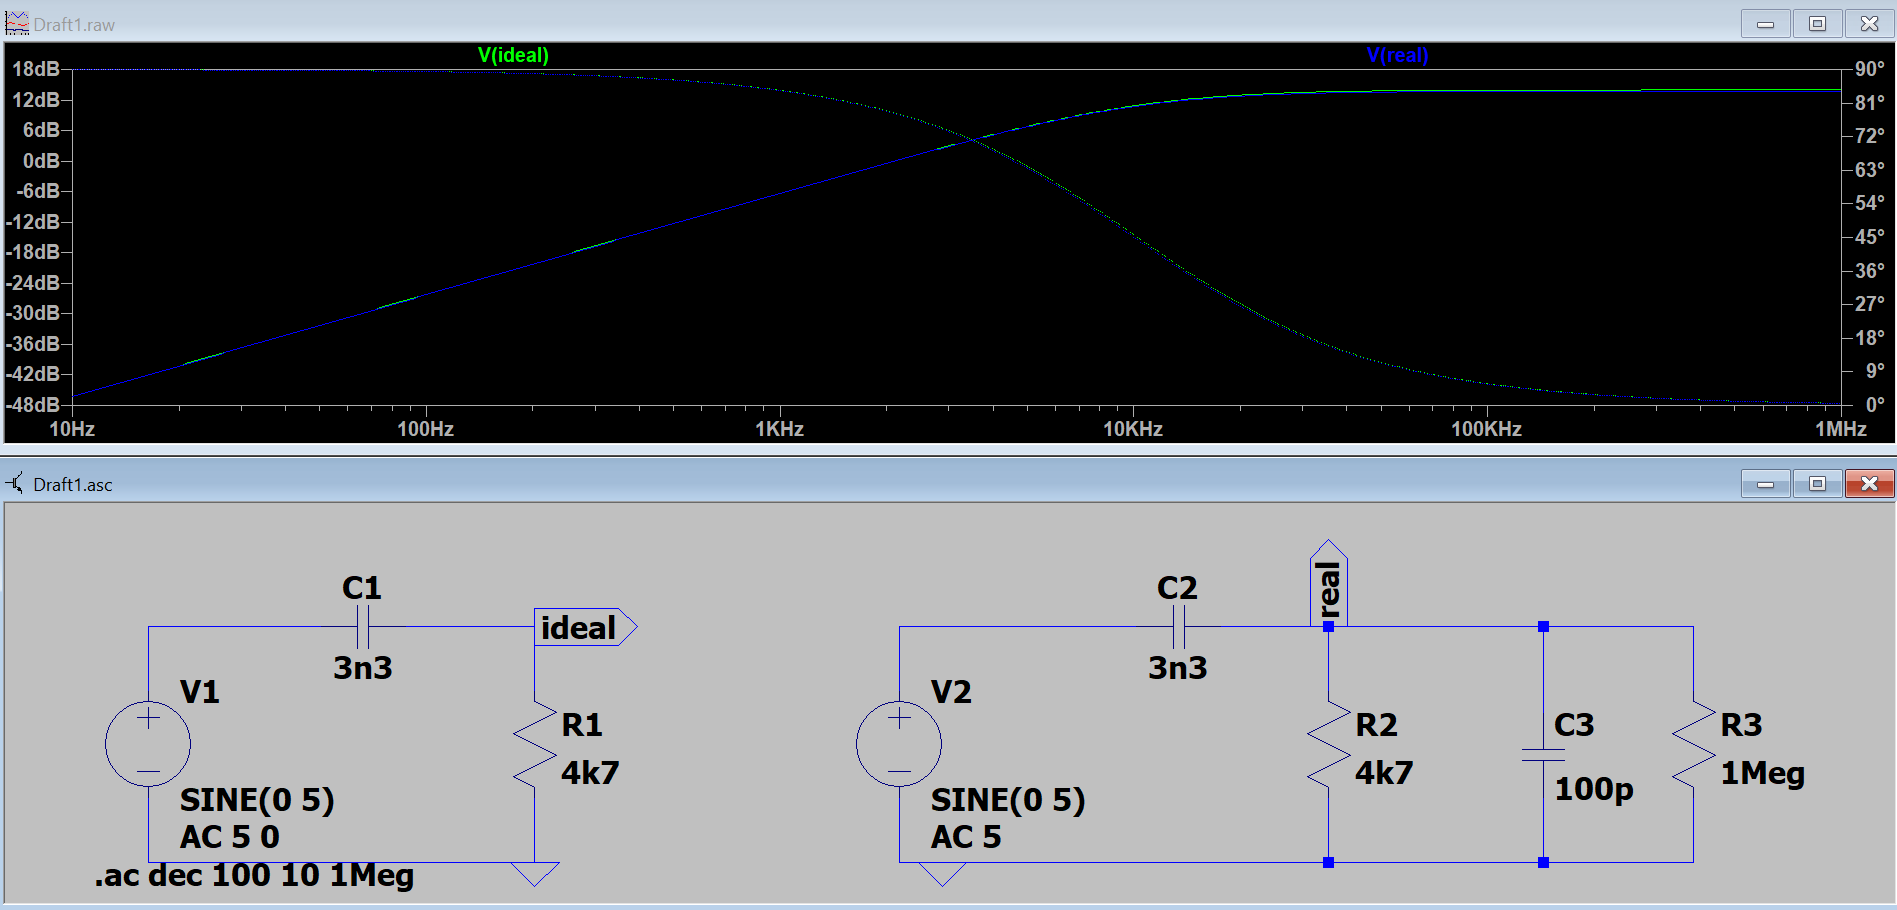
\includegraphics[width=0.5\linewidth]{item2_simulacion.png}
                \caption{Simulación del pasaaltos: ideal (izquierda) vs real(derecha)}
                \label{fig:pasaaltosSimulado}
            \end{figure}

            Luego, para los capacitores, las impedancias de ambos para $0,1f_0$, $f_0$ y $10f_0$ quedan como en la tabla \ref{table:impedanciasCapacivas} (observar anexo), sabiendo que $|Z_C|=\frac{1}{\omega C}$.

            Se puede ver que para frecuencias bajas y para la frecuencia de corte, el capacitor parásito de 100 pF genera una impedancia significativamente más alta que la resistencia de $ 4,7 k\Omega $, resultando en que la corriente circule por la misma. Por otro lado, para frecuencias mayores a la de corte, la impedancia generada por el capacitor de 3,3 nF es significativamente mayor a la de $470 k\Omega$, es decir que el capacitor de 100 pF resulta prácticamente insignificante en comparación al de 3,3 nF.

            \par Como se puede ver en las figuras \ref{fig:pasaaltosTeorico} y \ref{fig:pasaaltosMedido}, lo observado en el laboratorio coincide con lo esperado por las cuentas y la simulación.

%%%%%%nuevo%%%%%
\begin{figure}[H]
\centering

\begin{minipage}[t]{0.48\textwidth}
\centering
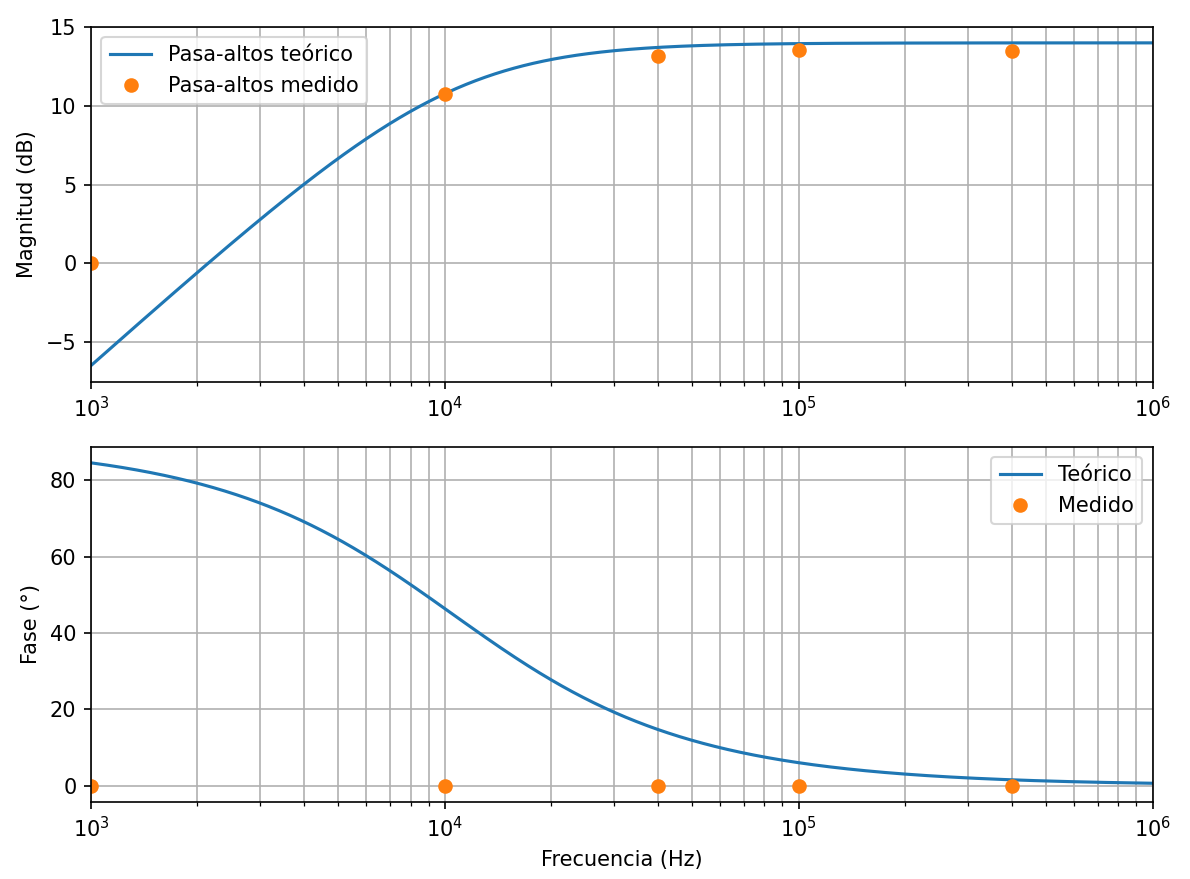
\includegraphics[width=\textwidth]{item2_bodeTeorico.png}
\captionof{figure}{Diagrama de BODE teórico del filtro pasa-altos con puntos medidos del módulo.}
\label{fig:pasaaltosTeorico}
\end{minipage}
\hfill
\begin{minipage}[t]{0.48\textwidth}
\centering
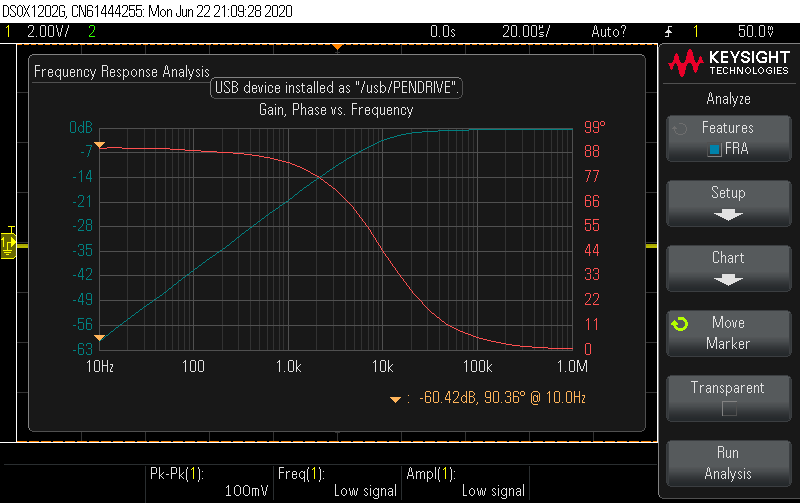
\includegraphics[width=\textwidth]{item2_bodeMedido.png}
\captionof{figure}{Diagrama de BODE medido}
\label{fig:pasaaltosMedido}
\end{minipage}

\end{figure}

%%%%%nuevo%%%%%

            Finalmente, se puede observar en la figura \ref{fig:Vr} que los valores obtenidos acorde a lo desarrollado en la sección \ref{vr} e ilustrados en la figura \ref{tab:vr_calculada} coinciden con la curva teórica del filtro pasa-altos.
            \begin{figure}[H]
                \centering
                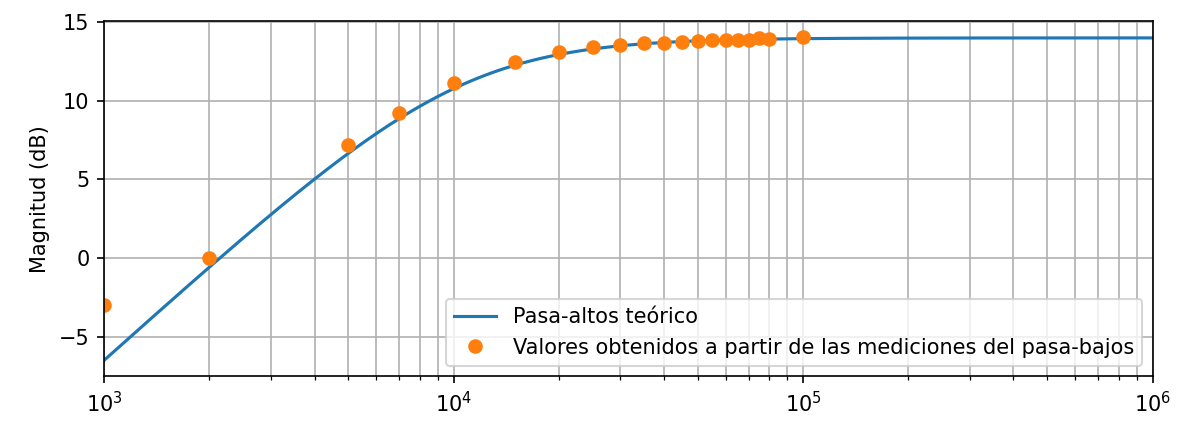
\includegraphics[width=0.5\linewidth]{pasaaltosVSvr.png}
                \caption{Pasa-altos teórico vs valores de Vr obtenidos acorde a lo desarrollado en el inciso 1.2.g}
                \label{fig:Vr}
            \end{figure}

        \subsubsection*{b) Alimentación con Señal Triangular}

        Como se puede ver en la figura \ref{fig:item2-triangular-bajo} y \ref{fig:item2-triangular-alto}, para frecuencias mucho menores a la
        de corte (10k) el filtro pasa-altos se comporta como un derivador (observar deducción en la subsección \ref{subsec:deduccion analitica derivador}).
        
        Para la frecuencia de corte, el capacitor de 3,3 nF no llega a cargarse completamente, dado
        que para $\tau = RC = 15,51 \mu s $ el tiempo de carga del circuito es
        $ 5\tau = 77,55 \mu s \approx 78 \mu s$, y un semiperíodo dura $ 50 \mu s $ (un tiempo menor al de carga).
        Cabe aclarar que a partir de esta frecuencia, para todas las frecuencias mayores el capacitor nunca
        va a llegar a cargarse completamente, ya que a mayor frecuencia menor período y menos van a durar los 
        semiperíodos en los que el capacitor se carga y se descarga.
        \par Para f=50 kHz, el tiempo que tiene el capacitor para cargarse es aun menor, y dado que la
        exponencial se parece a una recta para valores muy pequeños de la variable, que en este caso es el
        tiempo, lo que se ve en el osciloscopio es una curva muy parecida a una recta .

%%%%%nuevo%%%%%
\begin{figure}[H]
\centering

\begin{subfigure}{0.3\textwidth}
    \centering
    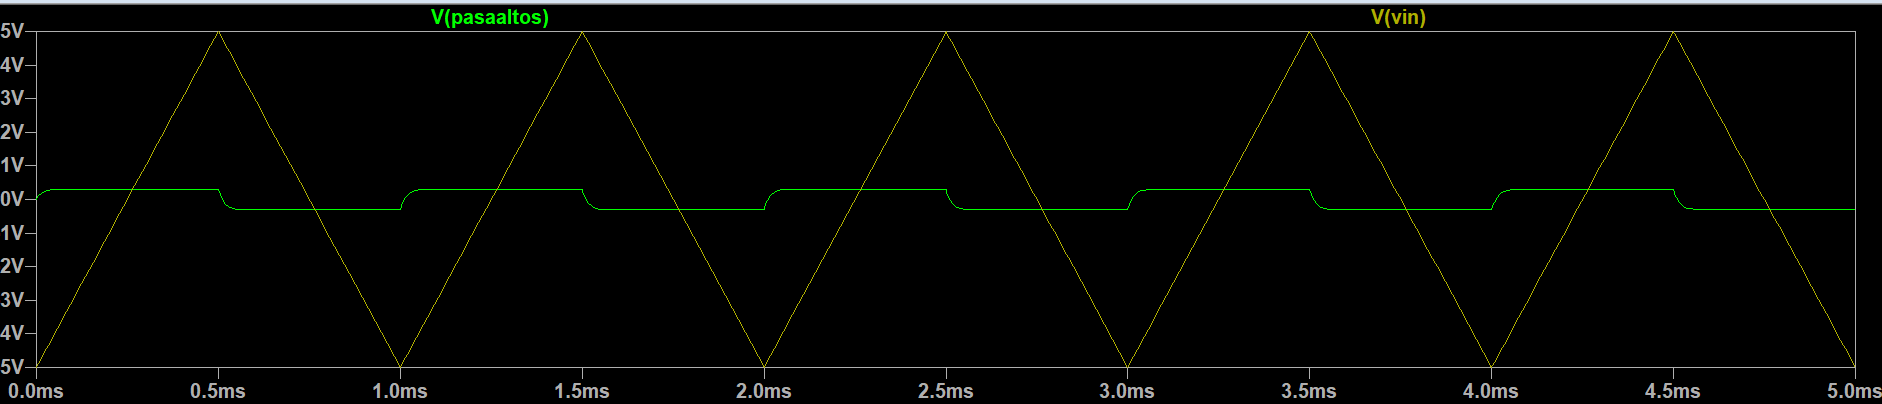
\includegraphics[width=\linewidth]{item2_triangular1k.png}
    \caption{$f=1\,\text{kHz}$}
\end{subfigure}
\hspace{0.01\textwidth}
\begin{subfigure}{0.3\textwidth}
    \centering
    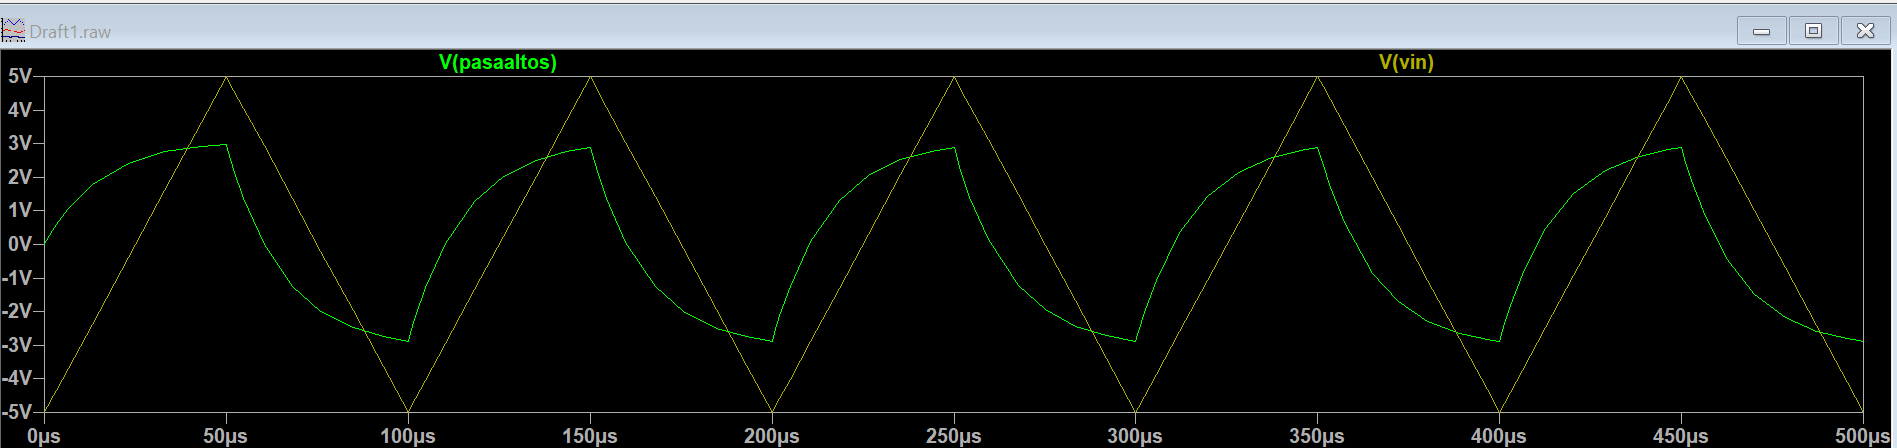
\includegraphics[width=\linewidth]{item2_triangular10k.png}
    \caption{$f=10\,\text{kHz}$}
\end{subfigure}

\vspace{0.15cm}

\begin{subfigure}{0.3\textwidth}
    \centering
    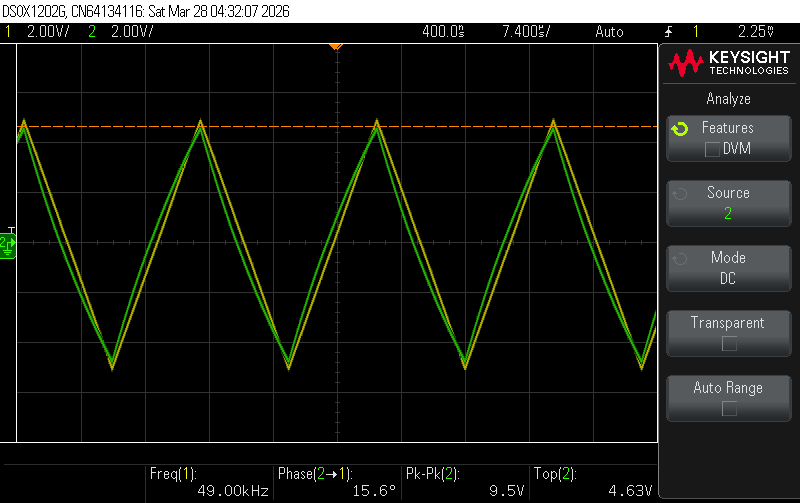
\includegraphics[width=\linewidth]{item2_triangular50k.png}
    \caption{$f=50\,\text{kHz}$}
\end{subfigure}
\hspace{0.01\textwidth}
\begin{subfigure}{0.3\textwidth}
    \centering
    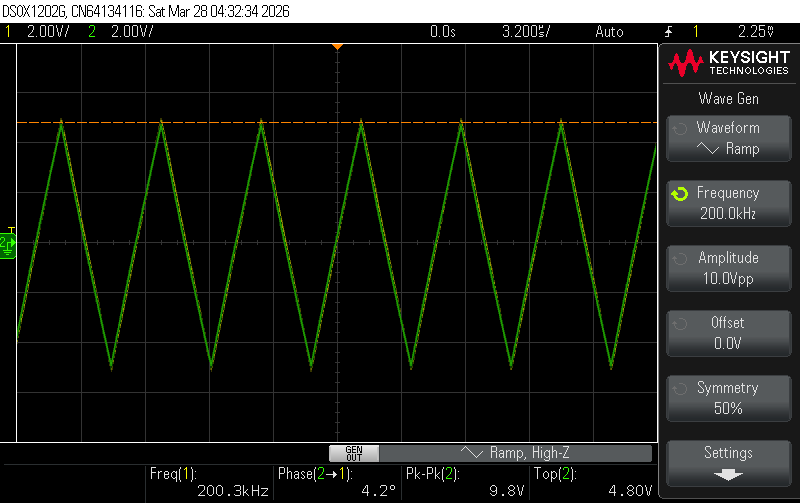
\includegraphics[width=\linewidth]{item2_triangular200k.png}
    \caption{$f=200\,\text{kHz}$}
\end{subfigure}

\caption{Respuesta del filtro pasa-altos ante una señal triangular para distintas frecuencias: 
(a) 1 kHz, (b) 10 kHz, (c) 50 kHz y (d) 200 kHz.}
\label{fig:item2-triangular}
\end{figure}


\section{Sincronización de instrumentos}

%%%%%%nuevo%%%%%%
\begin{figure}[H]
\centering

\begin{minipage}[t]{0.3\textwidth}
\centering
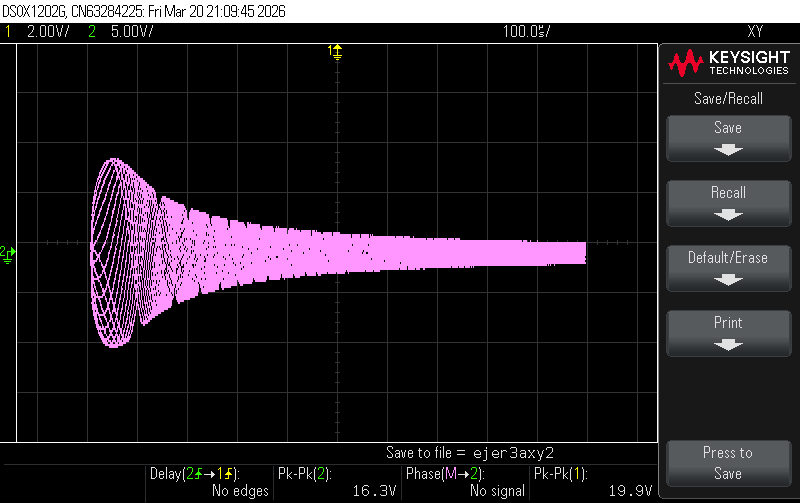
\includegraphics[width=\textwidth]{item3_modoXY.png}
\captionof{figure}{Barrido de la respuesta en frecuencia del filtro pasa-bajos en modo XY.}
\label{fig:barridoModoXY}
\end{minipage}
\hfill
\begin{minipage}[t]{0.3\textwidth}
\centering
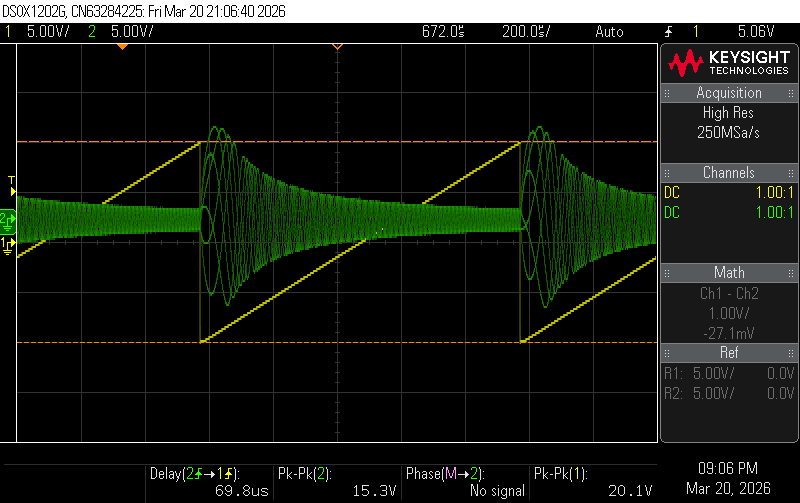
\includegraphics[width=\textwidth]{item3_modoNormal.png}
\captionof{figure}{Barrido de la respuesta en frecuencia del filtro pasa-bajos en modo normal.}
\label{fig:barridoModoNormal}
\end{minipage}

\end{figure}
%%%%%nuevo%%%%%%
    \subsubsection*{a) Usando modo XY del osciloscopio}
    Con el fin de estudiar el comportamiento en frecuencia del pasabajos previamente presentado
    utilizando un barrido, se emplearon dos generadores: en uno se generó la señal senoidal con la que
    se alimentó al circuito, y en el otro se generó una rampa. Ambas señales tenían igual período, y
    se sincronizó el trigger del osciloscopio con el canal correspondiente a la rampa, de manera que 
    cuando el trigger cruce cierto valor de la rampa se mostrara el barrido de ambas señales, 
    asegurando que esto ocurra una vez por cada período. Para que las señales no estén defasadas,
    se sincronizó el trigger de la señal senoidal con el de la rampa.

    Dado que la rampa está conectada al canal X, y su función es determinar la frecuencia de la señal
    de barrido, en este caso de la senoidal. Se puede ver que en la figura \ref{fig:barridoModoXY} que
    a mayor valor de la rampa, es decir mayor valor en el eje X, más grande es la frecuencia y más
    atenuada se ve la amplitud de la salida del circuito, como se esperaría de un pasa-bajos.
    
    \subsubsection*{a) Usando modo normal}


    En la figura \ref{fig:barridoModoNormal} se puede observar el mismo efecto descripto que para el modo 
    XY, pues al estar realizando un barrido cuanto mayor es la amgnitud de la rampa, mayor es la frecuencia
    de la senoidal de entrada, y más atenuada se ve la salida del circuito.



\section{Respuesta en frecuencia}
    % Medición con AC y BW limit vs datos del fabricante

\section{Utilización del hold off}
    % Señal compuesta y uso del hold off para ver parte triangular
    
    
    
    
    %%%%%%%%%%%%%%%%%%%%%%%%%%%%%%%%%%%%%%%%%
    
    %				ANEXO 
    
    %%%%%%%%%%%%%%%%%%%%%%%%%%%%%%%%%%%%%%%%%
\section{Anexo}

    \subsection{Osciloscopio digital y puntas de medición}

        El osciloscopio digital puede modelarse de forma aproximada como una impedancia de entrada compuesta por una resistencia de 1 M$\Omega$ en paralelo con una capacitancia parásita del orden de algunos pF (típicamente alrededor de 12 pF). Esta capacitancia no suele ser relevante a bajas frecuencias, pero empieza a afectar las mediciones cuando se trabaja en frecuencia más alta.

        Cuando se utiliza la punta en modo X1, la capacitancia total vista por el circuito aumenta bastante, llegando a valores del orden de 100 pF. Esto se debe principalmente al cable de la punta, que es coaxial, y por lo tanto se comporta como un capacitor distribuido (el conductor interno y la malla actúan como placas separadas por un dieléctrico). En este caso, el conjunto puede modelarse como una resistencia de 1 M$\Omega$ en paralelo con una capacitancia cercana a 100 pF, lo que puede modificar bastante la respuesta del circuito medido. %, como se muestra en la Fig.~\ref{fig:punta_x1}.

        Por otro lado, al utilizar la punta en modo X10, la propia punta introduce un divisor resistivo-capacitivo que compensa este efecto. Esto hace que la capacitancia equivalente vista por el circuito sea mucho menor (del orden de 10–15 pF) y que la resistencia de entrada efectiva aumente a aproximadamente 10 M$\Omega$. De esta forma, se reduce el efecto de carga sobre el circuito y se obtiene una medición más fiel. %, como se muestra en la Fig.~\ref{fig:punta_x10}.

\subsection{Deducción del los filtros}
\label{subsec:decuccion filtros}
Los filtros se pueden deducir usando un divisor resistivo. \par

En el caso del pasabajos, la deducción es la siguiente:

\begin{align*}
    v_{out} &= v_{in} \cdot \frac{\frac{1}{sC}}{R+ \frac{1}{sC}} \\
    \implies H(s) &= \frac{1}{SCR+1} \\
    H(s)&= \frac{1}{\frac{s}{\frac{1}{RC}} +1} 
\end{align*}

En el caso del pasaltos, la deduccion es la siguiente:

\begin{align*}
    V_{out} &= V_{in} \cdot \frac{R}{\frac{1}{sC}+R}\\
    H(s) &= \frac{sRC}{1+sRC}
\end{align*}

\subsection{Deducción del error de la frecuencia}
\label{subsec: Deducción del error de la frecuencia}
Para el error usaremos las derivadas parciales. \par

Recordemos que la frecuencia de ambos circuitos viene dada por la misma formula $f_0 = \frac{1}{2\cdot \pi \cdot C \cdot R} $. \par

Luego, la formula del error se deduce de la siguiente manera:

\begin{align*}
    \Delta f&= \sqrt{(\frac{\partial f }{\partial R} \cdot \Delta R)^{2} + (\frac{\partial f }{\partial C} \cdot \Delta C)^{2}}\\
    &= \frac{1}{2\cdot \pi \cdot R \cdot C} \cdot \sqrt{(\frac{\Delta R}{R})^2 + (\frac{\Delta C}{C})^2}\\
    & = f \cdot \sqrt{(\frac{\Delta R}{R})^2 + (\frac{\Delta C}{C})^2}
\end{align*}

\subsection{Deduccion desfase corriente y tensión del capacitor en el pasa bajos}
\label{subsec:desfase}

Primero es importante mencionar que como existe una malla, la corriente $I$ es la misma de todos los componentes. Luego:

\begin{align*}
    V_c&= I \cdot \frac{1}{j \cdot \omega \cdot C}\\
 \implies \angle V_c &= \angle I - 90^\circ \\
 \angle V_c - \angle I &= -90^\circ
\end{align*}


\subsection*{Tablas de datos}

%%%%%%tabla 1%%%%%
\begin{table}[H]
                    \centering
                    \renewcommand{\arraystretch}{1.1}
                    \begin{tabular}{ccccccc}
                    \toprule
                    \textbf{$f$} & \textbf{$|v|$ [V]} & \textbf{$|v_c|$ [V]} & \textbf{$\frac{v_c}{v}$ [dB]} & \textbf{$\Delta t$ [$\mu$s]} & \textbf{$\theta_{\Delta t}$} & \textbf{$\theta_{XY}$} \\
                    \midrule
                    500 Hz & 5,05 & 5,00 & -0,09 & 16,00 & -2,6$^\circ$ & 2,72$^\circ$ \\
                    1 kHz  & 5,05 & 5,00 & -0,09 & 15,10 & -5,4$^\circ$ & 5,67$^\circ$ \\
                    2 kHz  & 5,05 & 4,95 & -0,17 & 14,90 & -11,0$^\circ$ & 11,30$^\circ$ \\
                    5 kHz  & 5,05 & 4,50 & -1,00 & 14,50 & -26,0$^\circ$ & 25,90$^\circ$ \\
                    7 kHz  & 5,05 & 4,15 & -1,71 & 13,90 & -35,0$^\circ$ & 35,10$^\circ$ \\
                    10 kHz & 5,05 & 3,55 & -3,06 & 12,38 & -44,7$^\circ$ & 44,63$^\circ$ \\
                    15 kHz & 5,05 & 2,80 & -5,13 & 10,31 & -55,5$^\circ$ & 54,87$^\circ$ \\
                    20 kHz & 5,05 & 2,25 & -7,03 & 8,80 & -62,8$^\circ$ & 62,99$^\circ$ \\
                    25 kHz & 5,05 & 1,90 & -8,49 & 7,40 & -66,9$^\circ$ & 65,50$^\circ$ \\
                    30 kHz & 5,00 & 1,58 & -10,01 & -6,50 & -71,0$^\circ$ & 70,81$^\circ$ \\
                    35 kHz & 5,00 & 1,38 & -11,19 & -5,84 & -73,0$^\circ$ & 72,42$^\circ$ \\
                    40 kHz & 4,965 & 1,22 & -12,19 & -5,20 & -74,0$^\circ$ & 72,50$^\circ$ \\
                    45 kHz & 4,965 & 1,095 & -13,13 & -4,60 & -74,0$^\circ$ & 74,39$^\circ$ \\
                    50 kHz & 5,00 & 0,985 & -14,11 & 4,30 & -77,6$^\circ$ & 77,47$^\circ$ \\
                    55 kHz & 4,99 & 0,90 & -14,88 & -4,00 & -78,0$^\circ$ & 78,30$^\circ$ \\
                    60 kHz & 4,99 & 0,83 & -15,58 & -3,70 & -80,0$^\circ$ & 80,00$^\circ$ \\
                    65 kHz & 4,99 & 0,765 & -16,29 & -3,41 & -80,0$^\circ$ & 80,41$^\circ$ \\
                    70 kHz & 4,99 & 0,72 & -16,82 & -3,20 & -80,0$^\circ$ & 80,35$^\circ$ \\
                    75 kHz & 5,05 & 0,70 & -17,16 & 3,10 & -86,0$^\circ$ & 84,00$^\circ$ \\
                    80 kHz & 4,99 & 0,635 & -17,91 & -2,83 & -82,0$^\circ$ & 83,68$^\circ$ \\
                    100 kHz & 5,05 & 0,515 & -19,83 & 2,26 & -81,0$^\circ$ & 81,00$^\circ$ \\
                    \bottomrule
                    \end{tabular}
                    \vspace{0.3cm}
                    \caption{Respuesta en frecuencia del circuito pasa-bajos.}
                    \label{tab:pasa_bajos_freq}
                    \end{table}
  %%%%%%%%tabla1%%%%%%%%%%
  
  
  %%%%%%%%tabla 2%%%%%%%%%
  \begin{table}[H]
         \centering
        \renewcommand{\arraystretch}{1.1}
        \begin{tabular}{cccc}
        \toprule
        \textbf{Frecuencia} & \textbf{$|v|$ [V]} & \textbf{$|v_c|$ [V]} & \textbf{$|v_r|$ Calculado [V]} \\
        \midrule
        500 Hz & 5,05 & 5,00 & 0,71 \\
        1 kHz  & 5,05 & 5,00 & 0,71 \\
        2 kHz  & 5,05 & 4,95 & 1,00 \\
        5 kHz  & 5,05 & 4,50 & 2,29 \\
        7 kHz  & 5,05 & 4,15 & 2,88 \\
        10 kHz & 5,05 & 3,55 & 3,59 \\
        15 kHz & 5,05 & 2,80 & 4,20 \\
        20 kHz & 5,05 & 2,25 & 4,52 \\
        25 kHz & 5,05 & 1,90 & 4,68 \\
        30 kHz & 5,00 & 1,58 & 4,74 \\
        35 kHz & 5,00 & 1,38 & 4,81 \\
        40 kHz & 4,965 & 1,22 & 4,81 \\
        45 kHz & 4,965 & 1,095 & 4,84 \\
        50 kHz & 5,00 & 0,985 & 4,90 \\
        55 kHz & 4,99 & 0,90 & 4,91 \\
        60 kHz & 4,99 & 0,83 & 4,92 \\
        65 kHz & 4,99 & 0,765 & 4,93 \\
        70 kHz & 4,99 & 0,72 & 4,94 \\
        75 kHz & 5,05 & 0,70 & 5,00 \\
        80 kHz & 4,99 & 0,635 & 4,95 \\
        100 kHz & 5,05 & 0,515 & 5,02 \\
        \bottomrule
        \end{tabular}
        \caption{Tensión calculada sobre la resistencia en función de la frecuencia.}
        \label{tab:vr_calculada}
                    \end{table}
%%%%%%%%%%%%%%%%tabla 2%%%%%%%%%%%%%%%

%%%%%%%tabla3%%%%%%%%%%%%%
            \begin{table}[H]
                \centering
                \begin{tabular}{|c|c|c|c|}
                    \hline     & $0,1f_0$    & $f_0$           & $10f_0$       \\ \hline
                    $Z_{3,3n}$ & $47 k\Omega$ & $4,7 k\Omega$ & $470 k\Omega$ \\ \hline
                    $Z_{100p}$ & $1,55 M\Omega = 1545 k\Omega$ & $154,5 k\Omega$ & $15,45 k\Omega$ \\ \hline
                \end{tabular}
                \caption{Impedancias capacitivas para frecuencias centradas en la frecuencia de corte}
                \label{table:impedanciasCapacivas}
            \end{table}
 %%%%%%%%%%tabla3%%%%%%%%%%%%

\subsection*{Imagenes}

%%%%%%%%%%%%imagen 1%%%%%%%%%%%%%
                \begin{figure}[H]
                 \centering
                    \begin{minipage}{0.6\textwidth}
                            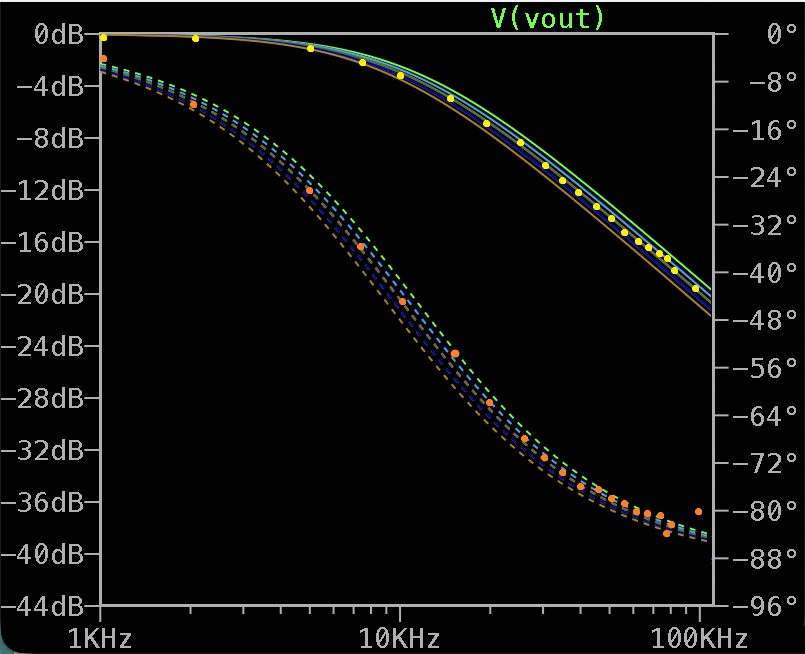
\includegraphics[width=\linewidth]{1.2d.png}
                            \caption*{Diagrama de Bode experimental sobre el teórico.}
                        \end{minipage}
                \end{figure}
%%%%%%%%%%%%imagen 1%%%%%%%%%%%%%

%%%%%%%%%%%%imagen 2%%%%%%%%%%%%%                        
                \begin{figure}[H]
                    \centering
                    \begin{tikzpicture}
                        % Eje principal (Magnitud / Ganancia)
                        \begin{semilogxaxis}[
                            width=10cm, height=5cm,
                            title={Ganancia y Fase vs. Frecuencia},
                            xlabel={Frecuencia [Hz]},
                            ylabel={Ganancia [dB]},
                            xmin=10, xmax=1000000,
                            ymin=-40, ymax=5,
                            ytick={-40,-35,-30,-25,-20,-15,-10,-5,0,5},
                            grid=both,
                            grid style={line width=.1pt, draw=gray!30},
                            major grid style={line width=.2pt,draw=gray!50},
                            axis y line*=left,
                            axis x line*=bottom,
                            ylabel near ticks,
                            % --- Ajustes de color para el eje Y izquierdo ---
                            y axis line style={teal},
                            ylabel style={teal},
                            yticklabel style={teal}
                        ]
                            % Curva de Ganancia
                            \addplot[
                                domain=10:1000000,
                                samples=200,
                                thick,
                                teal
                            ] {-10*log10(1 + (x/10000)^2)};
                            
                        \end{semilogxaxis}
                    
                        % Eje secundario superpuesto (Fase)
                        \begin{semilogxaxis}[
                            width=10cm, height=5cm,
                            xmin=10, xmax=1000000,
                            ymin=-96, ymax=12,
                            ytick={-96,-84,-72,-60,-48,-36,-24,-12,0,12},
                            ylabel={Fase [$^\circ$]},
                            axis y line*=right,
                            axis x line=none,
                            ylabel near ticks,
                            % --- Ajustes de color para el eje Y derecho ---
                            y axis line style={red},
                            ylabel style={red},
                            yticklabel style={red}
                        ]
                            % Curva de Fase Ajustada
                            \addplot[
                                domain=10:1000000,
                                samples=200,
                                thick,
                                red
                            ] {0.82 - atan(x/10000) + atan(x/35000000)};
                            
                        \end{semilogxaxis}
                    \end{tikzpicture}
                    \caption{Diagrama de Bode (ganancia y fase) modelado a partir de los datos del Auto-Bode.}
                    \label{fig:bode_tikz_final}
                \end{figure}
%%%%%%%%%%%%imagen 2%%%%%%%%%%%%%

%%%%%%%%%%%%imagen 3%%%%%%%%%%%%%                        
                    \begin{figure}[H]
                        \centering
                        % Primera fila: 100 Hz y 1 kHz
                        \begin{minipage}{0.48\textwidth}
                            \centering
                            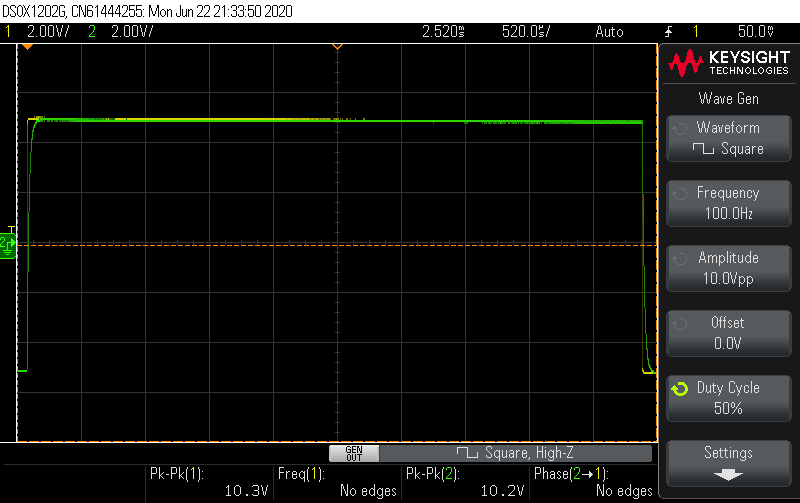
\includegraphics[width=\linewidth]{item1_cuadrada.png}
                            \caption*{a) $f = 100\text{ Hz}$}
                        \end{minipage}\hfill
                        \begin{minipage}{0.48\textwidth}
                            \centering
                            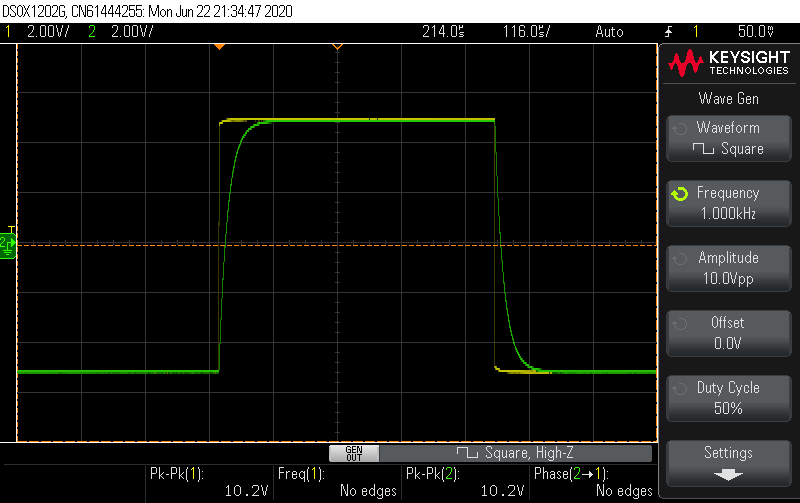
\includegraphics[width=\linewidth]{item1_cuadrada1.png}
                            \caption*{b) $f = 1\text{ kHz}$}
                        \end{minipage}
                        
                        \vspace{0.4cm}
                        
                        % Segunda fila centrada: 10 kHz
                        \begin{minipage}{0.48\textwidth}
                            \centering
                            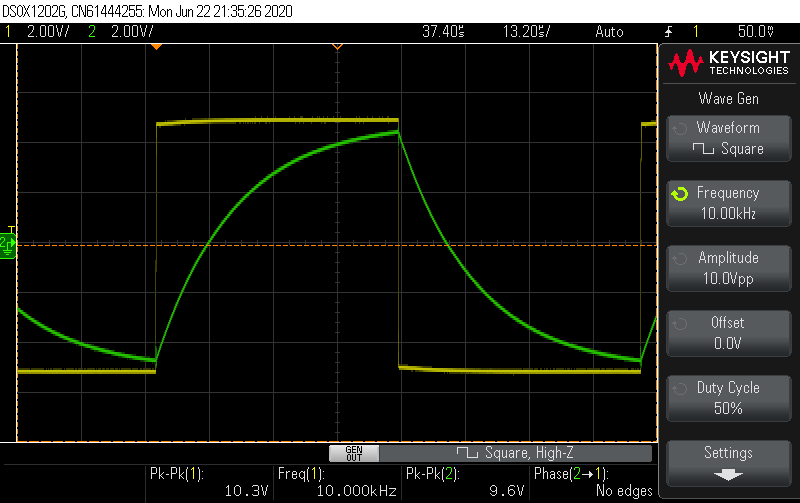
\includegraphics[width=\linewidth]{item1_cuadrada2.png}
                            \caption*{c) $f = 10\text{ kHz}$}
                        \end{minipage}
                        \caption{Respuesta del filtro pasa-bajos ante una onda cuadrada a distintas frecuencias. En amarillo se observa la señal de entrada y en verde la señal de salida sobre el capacitor.}
                        \label{fig:ondas_cuadradas}
                    \end{figure}
%%%%%%%%%%%%imagen 3%%%%%%%%%%%%%
 
\subsection*{Configuración de Puntas de Osciloscopios}
                    \begin{itemize}
    \item \textbf{Configuración con punta en modo $\times 1$:}
    La alta capacitancia del cable coaxial domina la respuesta del sistema. Para esta configuración, se obtuvo una frecuencia de corte medida de $f_{c1} = 300\text{ kHz}$. A partir de la relación $C_{p} = \frac{1}{2\pi R f_c}$, se calcula una capacitancia de:
    \begin{equation*}
    C_{p(\times 1)} = \frac{1}{2\pi \cdot 4650\,\Omega \cdot 300\cdot 10^3\text{ Hz}} \approx 114\text{ pF}
    \end{equation*}
    Este valor resulta coherente con el orden de magnitud esperado para una punta en $\times 1$ (típicamente $\approx 100\text{ pF}$), confirmando el severo efecto de carga que introduce el cable en mediciones directas.
    
    \item \textbf{Configuración con punta en modo $\times 10$:}
    Al activar el atenuador físico, la carga capacitiva sobre el circuito disminuye drásticamente, desplazando el polo del sistema hacia frecuencias más altas. En este modo, la frecuencia de corte medida se desplazó hasta $f_{c10} = 2\text{ MHz}$, resultando en una capacitancia de:
    \begin{equation*}
    C_{p(\times 10)} = \frac{1}{2\pi \cdot 4650\,\Omega \cdot 2\cdot 10^6\text{ Hz}} \approx 17,1\text{ pF}
    \end{equation*}
    Este resultado se aproxima notablemente al valor nominal esperado de una punta compensada (que suele rondar los $15\text{ pF}$).
                    \end{itemize}
                    Al analizar estos resultados, se observa que hay cierta capacitancia parásita del montaje: 
                    La pequeña diferencia entre los $17,1\text{ pF}$ calculados y los $15\text{ pF}$ teóricos se atribuye a la capacitancia parásita de la protoboard y las conexiones físicas, la cual se estima en el orden de los $2\text{ pF}$ adicionales.


%%% test%%

%%% test%%
        
\end{document}
